% USE XeLaTeX

\documentclass{beamer}
%% Possible paper sizes: a0, a0b, a1, a2, a3, a4.
%% Possible orientations: portrait, landscape
%% Font sizes can be changed using the scale option.
\usepackage[size=a1,orientation=portrait,scale=1.05]{beamerposter}


\usepackage[utf8]{inputenc}
\usepackage[T1]{fontenc}
\usepackage{libertine}
\usepackage[scaled=0.92]{inconsolata}
\usepackage[libertine]{newtxmath}


%% packages added by GG
\setbeamertemplate{caption}[numbered]  % enable numbering of figures in beamer-poster

\usepackage{lipsum,lineno}

\usepackage{multicol}
\usepackage{amsmath, amsthm, amsfonts}
\usepackage{amsfonts}
\usepackage{xcolor}
\usepackage{mathbbol}
\usepackage{amssymb}             % AMS Math
\DeclareSymbolFontAlphabet{\amsmathbb}{AMSb}%
\usepackage{bbm}


\usepackage{caption}
\usepackage{graphicx,subfigure}
\usepackage{floatrow}
\usepackage{booktabs} % more pro tables
\usepackage{tabularx} % tables for boundary conditions
\usepackage{multirow} % enchanted tables 
%\usepackage[shortlabels]{enumitem} % support letters for enumeration
\usepackage{ragged2e}  % to align / justify text

\usepackage{pifont}% http://ctan.org/pkg/pifont
\newcommand{\cmark}{\ding{51}}%
\newcommand{\xmark}{\ding{55}}%

%% GG styles

\newenvironment<>{redblock}[1]{
  \setbeamercolor{block title}{fg=white,bg=red!75!black}
  \setbeamercolor{block body}{fg=black,bg=white!25!red}
  \begin{block}#2{#1}}{\end{block}}
  
\newenvironment<>{blueblock}[1]{%
  \setbeamercolor{block title}{fg=white,bg=blue!75!black}%
  \begin{block}#2{#1}}{\end{block}}
  
\newenvironment<>{greenblock}[1]{%
  \setbeamercolor{block title}{fg=white,bg=green!50!black}%
  \begin{block}#2{#1}}{\end{block}}
  
%% end of GG stuff


\usepackage{cleveref}  % Warning: cleverref has to be loaded after hyperref!
% shortcuts from ŁŁW
\newcommand{\pr}[1]{\frac{\partial}{\partial #1}}
\newcommand{\rr}[2]{\frac{\partial #1}{\partial #2}}
\newcommand{\ppr}[1]{\frac{\partial^2}{\partial #1^2}}
\newcommand{\prr}[2]{\frac{\partial^2}{\partial #1\partial #2}}
\newcommand{\rpr}[2]{\frac{\partial^2 #1}{\partial #2^2}}
\newcommand{\rrr}[3]{\frac{\partial^2 #1}{\partial #2\partial #3}}

\newcommand{\R}{\mathbb{R}}
\newcommand{\E}{\mathbb{E}}
\newcommand{\Var}{\text{Var}}
\newcommand{\eq}{\text{eq}}
%\newcommand{\x}{\overline{x}}
\newcommand{\f}{\tilde{f}}
%===============================

\definecolor{VioletRed}{RGB}
%{127,127,127}% ccfd-grey
{0,26,102} % pw-blue
%{215, 0, 0} % red
\setbeamercolor{block title}{fg=VioletRed,bg=white}
\setbeamercolor{block body}{fg=black,bg=white}
\setbeamercolor{local structure}{fg=VioletRed}
\setbeamercolor{bibliography structure}{fg=VioletRed}
\setbeamercolor{bibliography item}{fg=black,bg=white}
\setbeamercolor{bibliography entry author}{fg=black,bg=white}
\setbeamercolor{bibliography item}{fg=black,bg=white}
\setbeamercolor{bibliography entry location}{fg=black} 
\setbeamercolor{bibliography entry note}{fg=black} 

\newenvironment<>{varblock}[2][\textwidth]{%
   \setlength{\textwidth}{#1}
   \begin{actionenv}#3%
     \def\insertblocktitle{#2}%
     \par%
     \usebeamertemplate{block begin}}
   {\par%
     \usebeamertemplate{block end}%
   \end{actionenv}}
   

\author[ggruszczynski@meil.pw.edu.pl]{\underline{G. Gruszczyński}$^{a,b}$, Ł. Łaniewski-Wołłk$^b$%, J. Szumbarski 
%\\ \texttt{sam@somewhere.edu}
}
%\author[sam \& joey]
%       {\parbox[t]{1.5in}{sam \\ \texttt{sam@somewhere.edu}} \and 
%        \parbox[t]{1.5in}{joey}
%       }
%ggruszczynski@meil.pw.edu.pl

%\institute{Institute of Aeronautics and Applied Mechanics \\ Warsaw University of Technology, Warszawa, Poland}


\institute
{
$^a$University of Warsaw, Interdisciplinary Centre for Mathematical and Computational Modelling\newline %\\[1em] 
$^b$Warsaw University of Technology, Faculty of Power and Aeronautical Engineering
%\texttt{e-mail address}
}


\subtitle{Application of thermal Cascaded Lattice Boltzmann Method \\ to 3D simulations in a high Prandtl number regime }


\addtobeamertemplate{headline}{} {
 \leavevmode
  \begin{columns}[T]
    \begin{column}{.15\linewidth}
        \vskip2cm
        \hskip1cm
        \hspace*{4.0em}
        
\includegraphics[width=1.1\linewidth]{Images/LOGO/Logo_icm_niebieskie.png}
    \end{column}
    \begin{column}{.7\linewidth}
         \vskip2cm
         \centering
         \usebeamercolor{title in headline}{\color{black}\Huge{\textbf{\inserttitle}}\\[0.5ex]}
         \vskip.5cm
         \usebeamercolor{subtitle in headline}{\color{black}\huge{\insertsubtitle}\\[0.5ex]}
         \vskip.5cm
         \usebeamercolor{author in headline}{\color{fg}\Large{\textbf{\insertauthor}}\\[1ex]}
         \usebeamercolor{institute in headline}{\color{fg}\large{\insertinstitute}\\[1ex]}
         \vskip1cm
    \end{column}
    \begin{column}{.15\linewidth}
        \vskip 2.1cm
        \begin{flushleft}
        \hspace*{6.5em}
        
\includegraphics[width=0.45\linewidth]{Images/LOGO/symbol-PW.pdf}
        \end{flushleft}
        \hskip1cm
    \end{column}        
   \vspace{1cm}
  \end{columns}
 \vspace{0.5in}
 \hspace{0.5in}\begin{beamercolorbox}[wd=47in,colsep=0.15cm]{black}\end{beamercolorbox}
 \vspace{0.1in}
}
\usepackage{hyperref}
\usepackage{cleveref}
\begin{document}
\begin{frame}[fragile]\justify%\centering

%%%%%%%%%%%%%%%%%%%%%%%% No Columns - Intro %%%%%%%%%%%%%%%%%%%%%%%%
\begin{columns}[T]
\begin{column}{.96\textwidth}
\begin{block}{Introduction}\justify
In this contribution, a 3D thermal Cascaded Lattice Boltzmann Method is presented. 
Improvements to the LB collision kernel for both thermal and hydrodynamics field is introduced, by transforming the operations into the central moment space. 
The relaxation of central moments is defined in a reference frame moving with the fluid.
Moreover, the moments of equilibria are calculated from continuous Maxwell-Boltzmann distribution, thus do not suffer from truncation error. 
As a consequence, CLBM enhances Galilean invariance, accuracy and stability of the method. 

The Prandtl number (Pr), is defined as a ratio of molecular diffusivity of momentum to the molecular diffusivity of heat. 
For common fluids (e.g. oil), the Pr is usually high, which means that heat diffuses much slower than the momentum and the thermal boundary layer is contained within the velocity boundary layer. 
To reduce the computational overhead, a D3Q7 lattice is commonly used as it is enough to handle first-order moments of the discrete Boltzmann equation to recover the macroscopic advection-diffusion equation, which describes the temperature field. 
Unfortunately, in a high Pr regime, the low value of numerical conductivity leads to numerical artefacts known as a `wiggles`. 
A natural remedy is to apply a lattice with a larger number of discrete velocities like D3Q27. 
It has been found, that to benefit from the usage of such a lattice, the commonly used cascaded relaxation scheme for advection-diffusion like equations needs to be modified to account for the higher-order moments of the thermal field.
To demonstrate the accuracy of the proposed collision kernel, a mesh dependence study of steady forced convection from a confined cylinder is performed for different values of Pr number and compared against high-quality FEM solution.
\end{block}

\end{column}
\end{columns}
\vspace{1em}
\begin{columns}[T]
%\begin{column}{.2975\textwidth}
\begin{column}{.32\textwidth}

\begin{block}{Heat Transfer in LBM} \justify
%\begin{multicols}{2}
%\begin{figure}[H]
%\includegraphics[width = 1 \textwidth]{Images/shs_structure.png} 
%\caption{Surface structure}
%\end{figure}
%\columnbreak 
%\begin{figure}[H]
%\includegraphics[width = 1 \textwidth]{Images/chemical_n_shape.jpg} 
%\caption{Coating vs structure}
%\end{figure}
%\end{multicols}
\textbf{Fixed Prandl Number problem}\\
Macroscopic variables can be recovered from the moments of DF:
\begin{align*}  
\textit{mass density: \hspace{1em}} \rho &= \int f(\boldsymbol{x} , \boldsymbol{\xi}, t, T) d^3 \xi \\
\textit{momentum density: \hspace{1em}} \rho \boldsymbol{u} &= \int  \boldsymbol{\xi} f(\boldsymbol{x} , \boldsymbol{\xi}, t, T) d^3 \xi \\
\textit{internal energy density: \hspace{1em}} \rho i&= \dfrac{1}{2} \int |\boldsymbol{\xi} - \boldsymbol{u}|^2 f(\boldsymbol{x} , \boldsymbol{\xi}, t, T) d^3 \xi
\end{align*}

Why \underline{not} extract the temperature from internal energy as $i=c_v T$ ? \\

Such an approach together with the SRT collision operator would lead to the \textit{fixed Prandtl Number problem} 
because thermal conductivity can not be tuned independently of kinematic viscosity. % \parencite{He1998a,Cercignani1988}.

There are three approaches to solve the issue:

\begin{itemize}
\item Multi Relaxation Time + Multispeed LBM (there are not enough moments on standard lattices). 
\item Introduce new distribution function, which can evolve in its own way, responsible for the energy field. 
\item Use LBM for hydrodynamic coupled with another solver (e.g. finite difference) for temperature field.
\end{itemize}

\end{block}

\begin{block}{(De)Coupling of N-S and Energy equations}
Physically, equations are coupled:
\begin{itemize}
\item Energy Eq. $ \rightarrow $ NS: equation of state $f(p,\rho,T) = 0 $. \newline 
Usually, ideal gas $p(\rho, T) = \rho R T = \rho c_s^2 $ is assumed for single phase LBM models.
\item NS $ \rightarrow $ Energy Eq.: kinetic energy + dissipation (viscous heating) and compression work.
\end{itemize}
In simplified models, the NS equation is decoupled from energy eq.
The equation of state has a constant temperature $p(\rho, T) = \rho c_s^2 = \rho R T_0 $ and the sound speed is fixed as $c_s = \sqrt{R T_0}$ . \linebreak
As a result, these models are incompressible. \newline
To account for thermal advection the Boussinesq approximation can be employed,
\begin{align*} 
%\rho(T) & \approx \rho_0 (1- \alpha_V (T-T_0)), \\
\boldsymbol{F}_{bouyancy} &= [\rho(T) - \rho_0] \boldsymbol{g} = - \boldsymbol{g} \rho_0 \alpha_V (T-T_0).
\end{align*}
\end{block}


\end{column}

%\begin{column}{.2975\textwidth}
\begin{column}{.605 \textwidth}
\begin{block}{Governing Equations}
Simulate an incompressible flow coupled with heat transfer problem.
\begin{multicols}{2}
\textbf{Hydrodynamics}\\
The continuity and momentum equations are,
\begin{eqnarray}  
\left\{
	\begin{array}{ll}
\frac{\partial \rho}{\partial t} + \nabla \cdot \rho \textbf{u} = 0 \\
\rho\left( \frac{\partial \textbf{u} }{\partial t} + \textbf{u} \cdot \nabla \textbf{u}\right) = -\nabla p + \nabla \cdot (\mu[ \nabla \textbf{u} + (\nabla \textbf{u})^\top]) + \textbf{F}
	\end{array}\nonumber 
\right.
\end{eqnarray}

\columnbreak 

\textbf{Energy-field}\\
The Enthalpy balance equation is:
\begin{align*}
\pr{t} (\rho c_p T ) + \nabla \cdot (\boldsymbol{u} \rho c_p T ) &= \nabla \cdot (k \nabla T)  + \dot{q} \nonumber %\label{eq:enthalpy_transfer_eq}
\end{align*}
`Advection - Diffusion` of  $H$ is solved on a separate D2Q9 lattice.% \\ \vspace{1.5em}
\end{multicols}
\end{block}


\begin{block}{Lattice Boltzmann Method - Algorithm} \justify
\begin{multicols}{2}
The raw moments and central moments are defined as,
\begin{eqnarray}
\Upsilon_{mn} &=& \sum_{\alpha}(e_{\alpha x})^m ( e_{\alpha y})^n f_{\alpha} \nonumber \label{eq:raw_mom_def} \\
\tilde{\Upsilon}_{mn} &=& \sum_{\alpha} ( e_{\alpha x} - u_x)^m ( e_{\alpha y} - u_y)^n f_{\alpha} \nonumber \label{eq:cm_mom_def}
\end{eqnarray}

\columnbreak

Density and velocity are interpreted as zeroth and first moment respectively,
\begin{eqnarray} 
\rho &=& \Upsilon_{00} = \sum_\alpha f_\alpha,  \nonumber % \hspace{2em} \text{- normalized pressure} 
 \\
\rho \textbf{u} &=& [u_x, u_y]^\top = [ \Upsilon_{10}, \Upsilon_{01}]^\top 
= \sum_\alpha f_\alpha \textbf{e}_\alpha + \frac{\textbf{F}}{2} \delta t. \nonumber 
% \hspace{2em} \text{- macroscopic velocity} 
\end{eqnarray}
\end{multicols}


\begin{flushleft}
\begin{multicols}{2}
\textbf{Hydrodynamics}\\
\textit{1} Initialize $ \boldsymbol{f}(\textbf{x}, t)  $, \\ \vspace{1.em}

\textit{2} Compute 
$\rho\textbf{u} = [u_x, u_y]^\top = [ k_{10}, k_{01}]^\top 
= \sum_\alpha f_\alpha \textbf{e}_\alpha + \frac{\textbf{F}}{2} \delta t \nonumber  $, \\ \vspace{1.em}

\textit{3} Compute \linebreak
$\boldsymbol{\tilde{\Upsilon}}(\boldsymbol{x},t)
=\mathbb{N}\mathbb{M}\textbf{f}(\boldsymbol{x},t)$, 
\hspace{1em}
$\boldsymbol{\tilde{\Upsilon}}^{eq}(\boldsymbol{x},t)=$..., \hspace{1em} 
$\tilde{\textbf{F}}(\boldsymbol{x},t)=$...,
\\ \vspace{1.em}
 
\textit{4} Collision  \linebreak
$\boldsymbol{\tilde{\Upsilon}}^{*}(\textbf{x}, t) =  
(\mathbbm{1} - \mathbb{S})\boldsymbol{\tilde{\Upsilon}} + \mathbb{S} \boldsymbol{\tilde{\Upsilon}}^{eq}  + (\mathbbm{1} - \mathbb{S}/2)\tilde{\textbf{F}}, 
$
\\ \vspace{1.em}

\textit{5} Streaming  \linebreak
$
\boldsymbol{f}(\textbf{x} + \textbf{e}\delta t, t + \delta t ) 
= \mathbb{M}^{-1} \mathbb{N}^{-1} \boldsymbol{\tilde{\Upsilon}}^{*}(\textbf{x}, t).
$ 


\columnbreak 
\textbf{Energy-field}\\
\textit{1} Initialize 
$ \boldsymbol{h}(\textbf{x}, t) $, \\ \vspace{1.em}
%\pause

\textit{2} % Use $ \boldsymbol{u}$ from hydrodynamics,  \\ \vspace{1.em}
Compute $ H = \sum_{\alpha} h_{\alpha}(\boldsymbol{x},t) $ \\ \vspace{1.em}%


\textit{3} Compute \linebreak
$\boldsymbol{\tilde{\Upsilon}}^{H}(\boldsymbol{x},t)
=\mathbb{N}\mathbb{M}\textbf{h}(\boldsymbol{x},t)$,
\hspace{1em}
$\boldsymbol{\tilde{\Upsilon}}^{H,eq}(\boldsymbol{x},t)=$...
\\ \vspace{1.em}
 
%%\pause
\textit{4} Collision \linebreak
$ \boldsymbol{\tilde{\Upsilon}}^{H,*}(\textbf{x}, t) = 
(\mathbbm{1} - \mathbb{S}^{H}) \boldsymbol{\tilde{\Upsilon}}^H+ \mathbb{S}^{H} \boldsymbol{\tilde{\Upsilon}}^{H, eq} 
$ 
\\ \vspace{1.em}
%
\textit{5} Streaming  \\
$
\boldsymbol{h}(\textbf{x} + \textbf{e}\delta t, t + \delta t ) 
= \mathbb{M}^{-1} \mathbb{N}^{-1} \boldsymbol{\tilde{\Upsilon}}^{H,*}(\textbf{x}, t).
$

%\end{block}
\end{multicols}
\end{flushleft}

\begin{figure}[H]
   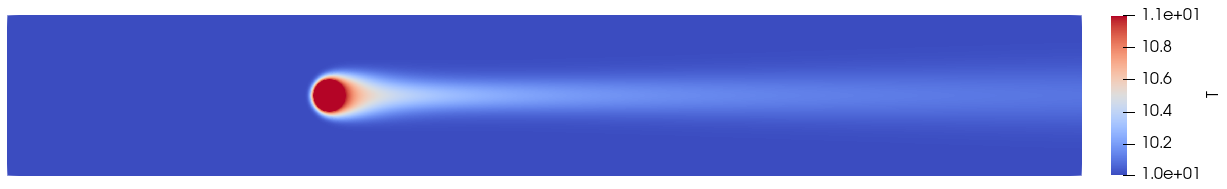
\includegraphics[width= 1 \textwidth]{Images/batch_HotKarman_Re10_Pr_10_D0_120_BR_1o5_nu_0o03_U_2o50e-03_2nd_order_bc_CM_HIGHER.png}
   \caption{Flow over a hot cylinder: Re=10 Pr=10 D=120}
   \label{fig:HotKarmanRe10Pr10D120}
\end{figure}

\end{block}
\end{column}
\end{columns}



\begin{columns}[T]
\begin{column}{.465\textwidth}
\begin{block}{Benchmark}
To validate the properties of the proposed LBM model, a flow around a hot cylinder (see \cref{fig:HotKarmanRe10Pr10D120}) has been simulated with different collision kernels and compared against FEM reference result. \newline


\begin{table}[H]
\begin{tabular}{llllllll}
Case-ID & $Nu_{CM}^{1st\; order\; bc} $ & $Nu_{CM}^{2nd\; order\; bc}$ & $Nu_{CM\; SRT}^{1st\; order\; bc}$ & $Nu_{CM\; SRT}^{2nd\; order\; bc}$ & $Nu_{CM\; TRT}^{1st\; order\; bc}$ & $Nu_{CM\; TRT}^{2nd\; order\; bc}$  & $Nu_{FEM}$ \\  \hline \hline
Pr10$_{small}$    & 5.26 	& 4.91 & 4.94 & 4.81 & 4.91	& 4.81	 & 4.82 \\
Pr10$_{medium}$   & 5.03 	& 4.84 & 4.87 & 4.81 & 4.86	& 4.81	 & 4.82 \\
Pr10$_{large}$    & 4.92 	& 4.83 & 4.84 & 4.81 & 4.83	& 4.81	 & 4.82    \\
Pr100$_{small}$   & 20.68 	& 14.75 & 10.64 & 10.20 & 10.66	& 10.27	 & 10.10    \\
Pr100$_{medium}$  & 15.87 	& 11.84 & 10.33 & 10.11 & 10.32	& 10.13  & 10.10    \\
Pr100$_{large}$   & 12.96 	& 10.64 & 10.20 & 10.09 &10.19	& 10.08	 & 10.10    \\
Pr1000$_{small}$  & 166.42 	& 102.27 & -135.45 & -138.08 & 27.09	& 24.58	 & 21.43   \\
Pr1000$_{medium}$ & 111.76 	& 62.52 & 22.75 & 21.78 & 22.73	& 21.84  & 21.43   \\
Pr1000$_{large}$  & 74.00 	& 40.47 & 21.87 & 21.38 & 21.84	& 21.37	 & 21.43  
\end{tabular}
\caption{Influence of kernel and BC on Nu number. \\
${1st\; order\; bc}$ = BB (hydrodynamics) + EQ (thermodynamics) \\
${2nd\; order\; bc}$ = IBB (hydrodynamics) + IABB (thermodynamics)
}
\label{tab:my-table}
\end{table}


\begin{table}[H]
\begin{tabular}{llllllllll}
Case-ID       & Lattice Size & Velocity set & Blockage Ratio & D   & U      & Pr   & Re & $\nu$   & $k$       \\  \hline \hline
Pr10$_{small}$    & 1000x150x3   & D3Q27Q27     & 1/5            & 30  & 0.01   & 10   & 10 & 3E-02 & 3E-03  \\
Pr10$_{medium}$   & 2000x300x3   & D3Q27Q27     & 1/5            & 60  & 0.005  & 10   & 10 & 3E-02 & 3E-03  \\
Pr10$_{large}$    & 4000x600x3   & D3Q27Q27     & 1/5            & 120 & 0.0025 & 10   & 10 & 3E-02 & 3E-03  \\
Pr100$_{small}$   & 1000x150x3   & D3Q27Q27     & 1/5            & 30  & 0.01   & 100  & 10 & 3E-02 & 3E-04  \\
Pr100$_{medium}$  & 2000x300x3   & D3Q27Q27     & 1/5            & 60  & 0.005  & 100  & 10 & 3E-02 & 3E-04  \\
Pr100$_{large}$   & 4000x600x3   & D3Q27Q27     & 1/5            & 120 & 0.0025 & 100  & 10 & 3E-02 & 3E-04  \\
Pr1000$_{small}$  & 1000x150x3   & D3Q27Q27     & 1/5            & 30  & 0.01   & 1000 & 10 & 3E-02 & 3E-05  \\
Pr1000$_{medium}$ & 2000x300x3   & D3Q27Q27     & 1/5            & 60  & 0.005  & 1000 & 10 & 3E-02 & 3E-05  \\
Pr1000$_{large}$  & 4000x600x3   & D3Q27Q27     & 1/5            & 120 & 0.0025 & 1000 & 10 & 3E-02 & 3E-05 
\end{tabular}
\caption{Case-ID: lookup table}
\label{tab:Case-ID_lookup_table}
\end{table}


\end{block}
\end{column}

\begin{column}{.46\textwidth}
\begin{block}{Influence of relaxation matrix}\justify
The general relaxation matrix for the advection diffusion equation can presented as:
\begin{align*}
 \mathbb{S}^{H} = diag\left([
 s_{000}, 
 s_{100}, 
 s_{010}, 
 s_{001}, 
 ...s_{ijk}...,
 s_{122},
 s_{212},
 s_{221},
 s_{222}
 ]\right) 
 \hspace{1em} \text{and} \hspace{1em}
 s^H = \frac{1}{\frac{k}{c_s^2 \delta t} + 1/2}
\end{align*}

\begin{itemize}
\item CM: The common approach for (central) moment based scheme for advection diffusion equation is to relax the first order moments only ($ s_{i+j+k = 1} =  s^H$), while the higher order moments are set to equilibrium ($ s_{i+j+k > 1} = 1$).
However, it turned out that such technique results in unacceptable `wiggles` for numerically low conductivities. %\newline
\item CM-TRT: The two-relaxation time approach requires the odd-moments to be relaxed with a common rate ($s_{odd} = s^H$), while the even moments are set to equilibrium ($s_{even} = 1$). %\newline
\item CM-SRT: The a single relaxation time can be obtained by setting $ s_{ijk} = s^H$.
\end{itemize} 
\vspace{1em}
\textbf{Conclusions}\\
To analyse flow of fluid having high Pr number, a lattice with large number of discrete velocities, like D3Q27, is necessary. 
Simulations on the D3Q7 lattice were unstable in the investigated regime.
Proper treatment of collision kernel seems to have a more important role than the application of a second-order BC to represent the cylinder.
The CM-TRT and CM-SRT kernels are superior to the kernels which relax first-order moments only. \\

The simulations were completed using the open-source TCLB solver available at: \newline 
{\fontfamily{lmtt}\selectfont
https://github.com/CFD-GO/TCLB
}
\vspace{2em}
\begin{figure}[H]
   
\includegraphics[width= 1 \textwidth]{Images/LOGO/Power-Eng_839x100-equal.jpg}
   %\caption{Flow over a hot cylinder: Re=10 Pr=10 D=120}
   %\label{fig:HotKarmanRe10Pr10D120}
\end{figure}

\begin{footnotesize}
"The program is co-financed from the European Social Fund under the Operational Program Knowledge Education Development, a non-competition project entitled "International scholarship exchange of doctoral students and academic staff" implemented as part of the Activity specified in the application for co-financing of the project no. POWR.03.03.00-00-PN13 / 18."
\end{footnotesize}

\end{block}
\end{column}
\end{columns}

%\begin{block}{References}
%\bibliographystyle{sbc}
%\bibliography{library.bib}
%\end{block}

\end{frame}
\end{document}


%%%%%%%%%%%%%%%%%%%%%%%% TEMPLATE %%%%%%%%%%%%%%%%%%%%%%%%

%\begin{columns}[T]
%\begin{column}{.46\textwidth}

%\begin{block}{Algorithm fluid}
%\lipsum[1]
%\end{block}
%\end{column}
%
%
%\begin{column}{.46\textwidth}
%\begin{block}{Algorithm fluid}
%\lipsum[2]
%\end{block}
%\end{column}
%\end{columns}
%%%%%%%%%%%%%%%%%%%%%%%% END OF TEMPLATE  %%%%%%%%%%%%%%%%%%%%%%%%

%%%%%%%%%%%%%%%%%%%%%%%% TEMPLATE %%%%%%%%%%%%%%%%%%%%%%%%
%\begin{block}{Sample...}
%\lipsum[1]
%\end{block}
%\begin{multicols}{2}
%\lipsum[2]
%\columnbreak 
%\lipsum[3]
%\end{multicols}
%%%%%%%%%%%%%%%%%%%%%%%% END OF TEMPLATE  %%%%%%%%%%%%%%%%%%%%%%%%

